\begin{appendices}

%Some Table of Contents entry formatting
\addtocontents{toc}{\protect\renewcommand{\protect\cftchappresnum}{\appendixname\space}}
\addtocontents{toc}{\protect\renewcommand{\protect\cftchapnumwidth}{6em}}

%Begin individual appendices, separated as chapters

\chapter{Experimental Equipment}
Per the handbook, numbering of figures and tables (and presumably equations) may be sequential throughout the document or prefixed with the chapter number.
The second option is used in this template, and so for appendices, a letter is used. 
For instance
\begin{align}
  a^{2} + b^{2} = c^{2}\,,
\end{align}
and for figures, see \cref{fig:AppendixTestFigure}.\footnote{%
Does it look familiar?
See also \cref{fig:IntensityVsWavelength}
}

\begin{figure}
  \centering
  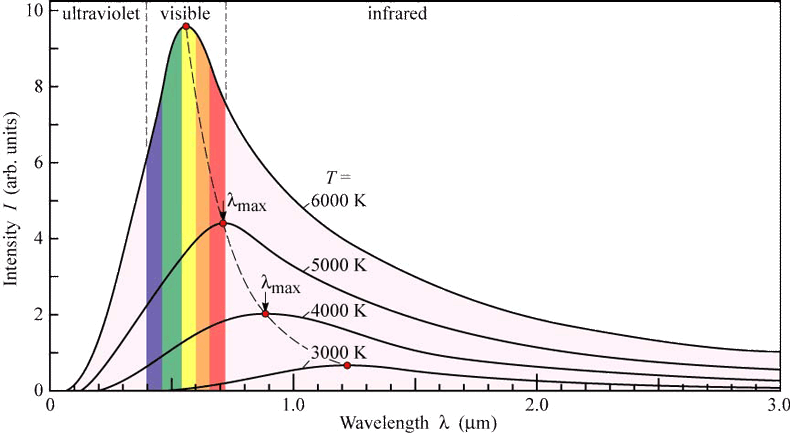
\includegraphics[width=0.75\linewidth]{figures/exampleFigure.png}
  \caption[The same damn figure]{Using this same graph to show how appendix figures are handled.}
  \label{fig:AppendixTestFigure}
\end{figure}

\section{Section of Appendix}

\chapter{Data Processing}
Lorem ipsum dolor sit amet, consectetur adipiscing elit, sed do eiusmod tempor incididunt ut labore et dolore magna aliqua. Ut enim ad minim veniam, quis nostrud exercitation ullamco laboris nisi ut aliquip ex ea commodo consequat. Duis aute irure dolor in reprehenderit in voluptate velit esse cillum dolore eu fugiat nulla pariatur. Excepteur sint occaecat cupidatat non proident, sunt in culpa qui officia deserunt mollit anim id est laborum.

\end{appendices}